\documentclass[tikz,border=50mm]{standalone}
% !TeX program = luatex

%===This is the preambule I call in every file===

\usepackage{tikz}
\usepackage{xcolor}
\usepackage{pgfplots}
\usepackage{circuitikz}
\usepackage{tikz-3dplot}
\pgfplotsset{compat=newest}
\usetikzlibrary{arrows.meta, shapes.geometric, positioning, perspective, patterns.meta, decorations.pathreplacing, decorations.pathmorphing, decorations.markings, patterns, arrows.meta, shapes, shapes.geometric, decorations.text, angles, quotes,calc, 3d, math, circuits.ee.IEC,hobby, knots, intersections, through}


%=== The Euler Med Logo ===
%=== i.e. My signature ===

\usepackage{amsmath, amsfonts}
\makeatletter
\newcommand*\eulermed{{
\scalebox{3.3}{$\mathbb{E}$}\kern-1pt \scalebox{1.5}{u$\ell\varepsilon\rho$}\kern-55pt
\raisebox{19pt}{\scalebox{1.5}{$\mathcal{M}\varepsilon\delta$}}}
\@}
\makeatother

\begin{document}
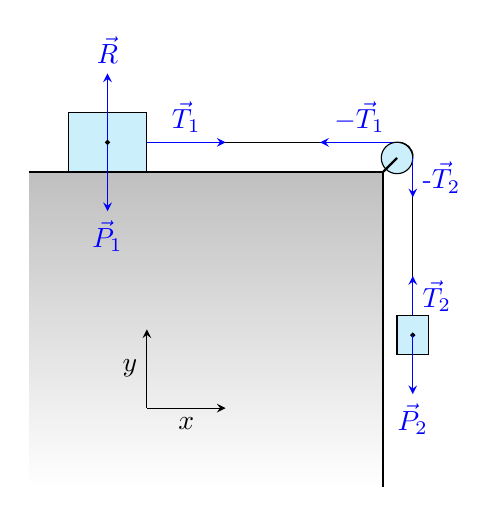
\begin{tikzpicture}[>=stealth]
\filldraw[top color=lightgray, bottom color=white, draw = white] (0,0)rectangle(4.5,4);
\draw[thick] (0,4)--(4.5,4)--(4.5,0);
\begin{scope}[shift={(0.5,4)}]
\filldraw[cyan, opacity=0.2] (0,0)rectangle(1,0.75);
\draw[black] (0,0)rectangle(1,0.75);
\filldraw[blue, ->] (0.5,{0.75/2})--(0.5,-0.5) node[below] {$\vec{P}_1$};
\draw[blue, ->] (0.5,0)--(0.5,1.25) node[above] {$\vec{R}$};
\filldraw[black] (0.5,{0.75/2})circle(0.025);
\draw[] (1,{0.75/2})--(4.2,{0.75/2});
\draw (4.2,{0.75/2})arc[start angle=90, end angle=0, x radius =0.18cm, y radius =0.18cm];
\draw[blue,->] (1,{0.75/2})--(2,{0.75/2}) node[above, midway] {$\vec{T}_1$};
\draw[blue, ->] (4.2,{0.75/2})--(3.2,{0.75/2}) node[above, midway] {$-\vec{T}_1$};
\end{scope}
\begin{scope}[shift={(4.5,4)}]
\filldraw[cyan, opacity=0.2] (45:0.25)circle(0.2);
\draw[] (45:0.25)circle(0.2);
\draw[thick] (0,0)--(45:0.25);
\begin{scope}[shift={(45:0.25)}]
\draw[] (0.2,0)--(0.2,-2);
\filldraw[cyan, opacity=0.2] (0,-2.5)rectangle(0.4,-2);
\draw[] (0,-2.5)rectangle(0.4,-2);
\filldraw[] (0.2,-2.25)circle(0.025);
\draw[->,blue] (0.2,-2.25)--(0.2,-3) node[below] {$\vec{P}_2$};
\draw[->,blue] (0.2,-2)--(0.2,-1.5) node[right, midway] {$\vec{T}_2$};
\draw[->,blue] (0.2,0)--(0.2,-0.5) node[right, midway] {-$\vec{T}_2$};
\end{scope}
\end{scope}
\draw[->] (1.5,1)--(1.5,2) node[midway, left] {$y$};
\draw[->] (1.5,1)--(2.5,1) node[midway, below] {$x$};
\end{tikzpicture}
\end{document}
